\section{Segregated Byzantine Agreement}
\label{sec:SBA}

The \textrm{Dusk} blockchain is built upon a novel consensus mechanism, called \textit{Segregated Byzantine Agreement} (SBA$\large\star$), engineered to provide the best possible tradeoff between security, efficiency and flexibility. 

SBA$\large\star$ complements the idea of \textit{Cryptographic Sortition,} \textit{Player Replaceability} and \textit{Ambiguity Resilience} (firstly introduced by the BA$\large\star$ consensus developed by Micali and the MIT CSAIL \cite{algorand}) with the new concepts of \textit{stealth time-locked transactions} as a method for Sybil resistance and \textit{non-interactive verifiable shared secret} scheme to implement a simple but secure $\textrm{(t,n)-threshold secret}$ sharing for keeping sortition auditable solely by a rotating set of \textit{pre-block Verifiers}.

In order to both improve network and block-generation efficiency and privacy of transacting peers, SBA$\large\star$ allows only normal transactional nodes to compete for block-generation, while it restricts the computationally and network intensive tasks associated with verification, voting and notarisation (VVN operations) to non-transactional nodes called \textit{Provisioners}. Provisioners harden the \textrm{Dusk} Blockchain by decreasing network communications across VVN operations, improving the time-to-finality through a notarisation process, decreasing the probability of network partitioning and contributing to the overall availability of \textrm{Dusk} Network.

Furthermore, they contribute distributed storage infrastructure in the \textrm{Dusk} On- Offline File Transfer, and enable runtime payments of high QoS transmission by handling \textit{state channels} for communicating peers through a novel mechanism of Secure Tunnel Switching.

\paragraph{BA$\large\star$}

Cryptocurrencies powered by message-passing Byzantine Agreement (BA$\large\star$), use cryptographic sortition in order to carry out the functionalities of block proposals, validations and subsequent insertion into a tamperproof sequence of blocks.

In its essence, each node of the network, while collecting (and further relaying) pending transactions, runs a computationally lightweight process that yields in a pseudo-random fashion which role such node should assume in the operations of production and validation of a new block. The great advantage of BA$\large\star$ compared to other consensus mechanisms based upon \textit{proof-of-work} or \textit{proof-of-stake}, lays primarily in avoiding any possibility of forking the Blockchain and thus preventing any ambiguity about which branch will become the dominating one.

This translates into the appealing property of achieving transaction "finality" as soon as consensus is reached for a block. In the best case scenario this happens after 2 rounds of non-interactive sortition. In the worst case scenario (weak network synchrony controlled by adversaries for a long but  bounded period of time), BA$\large\star$ achieves block finality after 9 rounds.

BA$\large\star$ consensus is a very convincing engine for powering open cryptocurrencies which do not require privacy. The election of Block Generator and Block Voter requires the total weights available in the system and each \textit{sortition candidate}'s balance to be public and known by all peers in order to allow blocks proposed by higher priority members to be propagated within the network and validated by multiple voting committees.

This is problematic for a privacy-oriented digital currency such as \textrm{Dusk} which strives to protect the data of the transacting actors. SBA$\large\star$ therefore focuses primarily on the privacy of transactional nodes while keeping auditable (but not public) only essential information about nodes participating in block generation, validation and notarisation.

\subsection{Consensus Outline}

The BA$\large\star$ algorithm has been developed in a direction unsuitable for \textrm{Dusk} because transactions are supposed to be propagated in clear, nodes do not keep private state except their private keys and there is no measure to prevent every node in the network to learn of every other node's balance, IP address and, ultimately, providing a mere pseudonimity to protect their identity.

We propose here a new approach that evolves BA$\large\star$ into what we call SBA$\large\star$ (as in \textit{Segregated Byzantine Agreement}$\large\star$) which finally renders the consensus mechanism an outstanding choice for privacy-oriented currencies (such as \textrm{Dusk}) due to its quick finality mechanism, minimal amount of computation required and speed in block production.

SBA$\large\star$ foresees different subsequent cyclic phases, all of which are non-interactive, with the sole exception of the \textit{Validation}, where the $\textrm{NIVSS\_Reconstruct}$ requires $O(1)$ communications to complete.
\paragraph*{Block Generation Sortition} Run by nodes with a time-locked stake called \textit{Block Generator} candidate (or simply a "\textit{candidate}"). During this phase the candidates run the VRF, calculate their priority, run the Non-Interactive Verifiable Shared Secret Protocol and propagate a \textit{pre-block} (which is a block proposal that still needs to get through various round of consensus and gets decorated with additional meta-data along the way) together with the various proofs.

\paragraph*{Default Block Generation Sortition} 
\textit{Run by Provisioners in parallel to the Block Generation Sortition}. In the eventuality that the Block Generation Sortition produces no \textit{candidate} with priority higher than zero or the Validation phase fails, Provisioners run the classic BA$\large\star$ Sortition algorithm to supply a \textit{default pre-block}.  
\paragraph*{Validation}
\textit{Run by a subset of Provisioners called Verifiers}. \textit{Verifiers} run the \textit{Secret Reconstruction Protocol}, validate the priority information of the highest priority candidate and either sign on the pre-block proposal of the \textit{candidate} or a \textit{default pre-block}. Additionally, the \textit{Verifiers} validate the witness $wit_P$ of candidate Provisioners committing their stake to the \hyperref[sec:Cryptographically-Committed-Provisioners]{Accumulator} if any. In this case, this information gets added to the pre-block
\paragraph*{Voting}
\textit{A number of rounds each of which run by a different subset of Provisioners called Voters}. BA$\large\star$ proves that the amount of round is optimistically 4 for a strongly synchronous network and 9 for a weakly synchronous one with a strong adversarial presence controlling the network (albeit for a finite period of time)
\paragraph*{Notarization}
\textit{The Voters which reached voting consensus on the pre-block are called Notaries}. The public key of the \textit{Notaries} are added to the pre-block and they play the role of \textit{Verifiers} in the next block's Validation phase. The pre-block is finally turned into an official block by the \textit{Notaries} by adding \hyperref[sec:Block-Reward]{the Block Reward information}.

\subsection{Verifiable Random Function}
\label{Verifiable-Random-Function}
The cryptographic sortition is implemented through the so-called Verifiable Random Function (VRF). Formally, for a generation algorithm $G\small{EN}$ producing the key pair $(P_k, S_k)$, a proving algorithm $P\small{ROVE}_{Sk}\normalsize(x)$ which outputs a pair of function value and proof of correctness ($F_{Sk}(x), \pi_{Sk}(x)$), a \textbf{VRF} is a function for which it exists a verification algorithm $V\small{ER}_{Pk}\normalsize(x, y, \pi)$ which verifies that $y=F_{Sk}(x)$ using proof $\pi$.

In practice a node running a VRF can prove the output it received by propagating $\pi$ together with the VRF result. This way a node, by running a VRF and communicating its output, can convince its peers in a non-interactive fashion (meaning without talking to anyone else in the network) whether he has been selected by "the cryptographic sortition" to play a specific role in the current block creation round.

The roles are either \textit{Block Generator\textit} or \textit{Block Verifier}. The elected node will then proceed to perform the steps foreseen by its role independently from all the other nodes (regardless of their role) and thus propagate the result of such operations to the network together with their allotment proof as outputted by the VRF. The nodes forfeit their role and become irrelevant to the consensus as soon as they communicate with the network. This way, the algorithm makes it virtually impossible for an adversary to target nodes participating in the block election or transaction validation. Only a small fraction of the nodes each round get randomly selected.

The likelihood of positive VRF output depends on a weight correlated to the amount of digital currency committed by a node. In \textit{BA$\large\star$} this is the public balance of each node, in SBA$\large\star$ this depends on the sortition role (i.e. Block Generators commit a payment while Provisioners commit a stake). Regardless of the type of commitment, the weight mechanism is used to prevent Sybil attacks since it renders probabilistically and economically disadvantageous for a node to replicate itself over several different Sybil processes, since such behaviour would actually decrease its chance of winning the ballot.

\begin{figure*}
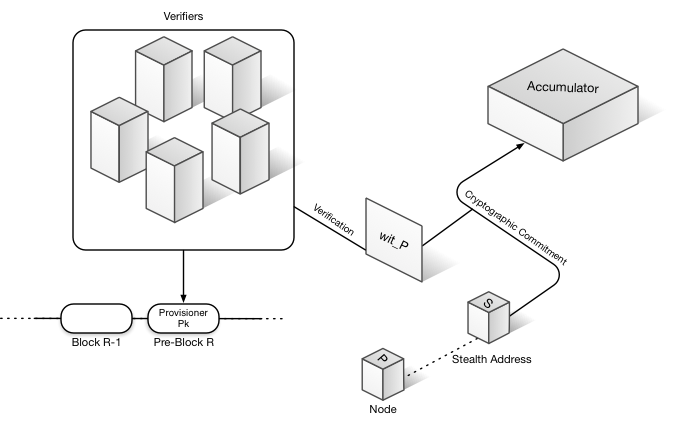
\includegraphics[scale=0.5]{Provisioners}
\caption{Provisioners setup}
\end{figure*}

\subsubsection{VRF And Sortition Procedure}

Through VRF sortition, a number of Block Generator candidates are selected each round. The candidates propagate their proposed block together with the VRF output, which includes the proof of winning the sortition together with the priority given by the digital currency balance of the node. Peers collect and propagate gossiped packets, forwarding solely the message with the highest priority and discarding all the others. The amount of time peers are supposed to collect messages is usually part of the protocol configuration and is suggested to be 5 seconds.

At the end of this period, peers which did not receive a message propagate an empty block (which is a perfectly valid outcome of the consensus). From a security perspective, an adversary could orchestrate an attack by deceiving peers into proposing different blocks. However, this attack would fail unless the adversary would have the highest priority in a round and if the number of honest Provisioners are also less then 2/3rd.

\subsection{Cryptographically Committed Provisioners}
\label{sec:Cryptographically-Committed-Provisioners}
One approach to protect the stake information was the employment of Order Preserving Encryption and Homomorphic Cypher \cite{alec}, which would have theoretically allowed for priority comparison without revealing the balance of the different nodes. This approach however has been discarded because it is susceptible to binary search attack. In fact, by exposing priority information, any attacker with access to the oracle could ultimately obtain information about the original balance of a node simply by performing multiple comparisons with the hash of a known number. Additionally, every node in the network is required to perform validation on the packets it receives.

Since the priority of the Block Generator is an input parameter for validating its VRF’s output, the measures required to provide access to such datum in a secure setting would result in an unacceptable degradation of performance and increase in complexity.

Instead, in the attempt to obtain the best trade-off between efficiency and anonymity, the system restricts the opportunity to perform VVN operations solely to non-transactional nodes called \textit{Provisioners} organized in elected subsets which form different committees throughout the algorithm rounds. In order to be eligible to be a Provisioner, a node $P$ uses a non-interactive \hyperref[sec:Cryptographic-Accumulator]{cryptographic commitment} to bind a predefined minimum amount of \textrm{Dusk} coins $C$ into a collective anonymous escrow and creating a $spend$ transaction toward a \textit{stealth address} obfuscating $P$'s address. Such $spend$ transactions are kept concealed until the node is ready to cash back its stack and quit its role as Provisioner.

The system verifies through an efficient (i.e. within \textit{polynomial-time}) \textit{non-interactive zero knowledge proof}  $wit_M$ that $P$ actually committed its stack in the Accumulator. This means that as soon as the Provisioner commits its stake to the Accumulator, it announces itself as a Provisioner to the network by gossiping its public key, its \textrm{Dusk} Network Address and $wit_P$. The drawback of relying on a trusted setup is circumvented by using the RSA-2048.

Also, the notoriously big size of spend proof (estimated to be 45kb in the Zerocoin whitepaper \cite{zerocoin}) is not problematic in the case of Provisioners since their stake is meant to be in a long-term escrow. This is easily enforceable at protocol level.

\subsection{Non-Interactive Verifiable Shared Secret Protocol}

Verifiable Secret Sharing (VSS) is a cryptographic protocol designed to allow a dealer to decompose a secret in $n$ fragments and share them publicly to $n$ peers (players) so that only a subset (\textit{threshold}) $t$ or those fragments are needed to reconstruct the original secret. In a VSS, through the addition of auxiliary information, players can verify reception of a "valid" fragment without acquiring any knowledge of the initial secret.

The Non-Interactive Verifiable Secret Sharing Protocol is the \textrm{Dusk} variation of the Simplified VSS protocol of Gennaro, Rabin and Rabin \cite{grr}. In our protocol, the \textit{dealer} does not communicate directly with the \textit{players} but can only rely on multiple untrusted message relayers as it is the case using the \textrm{Dusk} gossip protocol. The protocol foresees a \textit{sharing phase} () and a \textit{Reconstruction Phase}. The constant term $s$ of $f(x)$ is the secret. The second polynomial $r(x)$ is used to generate $t$ independent random strings used to commit to the shares.

The verification performed by player $P_i$ after decrypting its share $S_i$ from the share vector $S$, with its own private key $sk_i$ is trivially to recompute $\mathcal{A}_i = \mathcal{C}(\alpha_i, \rho_i)$ and check that the equation holds. $\mathcal{C}(x, r)$ is a commitment hash function such as $\textrm{Skein}$ or $\textrm{SHA-3}$.

    \begin{algorithm}
        \caption{Share secret in a verifiable and non-interactive way}
        \begin{algorithmic}[1]
            \Procedure{NIVSS\_Share}{$s, V$} \Comment{$s$ is a secret, $V$ a list of $n$ Verifiers $pk$}
                \State $f(x) = s \space + a_1x^1 + .. + a_tx^t$ \Comment{$f(x)$ is a random polynomial}
                \State $r(x) = r_0 + r_1x^1 + .. + r_tx^t$ \Comment{$r(x)$ is a random polynomial}
                \State $S = \{\}$
                \State $\mathcal{A} = \{\}$
                \For{each player $i$ in $V$}
                	\State $(\alpha_i, \rho_i) \leftarrow (f(i), r(i))$
                	\State $S_i \bigcup = \{Enc_{pk_i}(\alpha_i, \rho_i)\}$
                	\State $\mathcal{A}_i \bigcup = \{\mathcal{C}(\alpha_i, \rho_i)\}$
                \EndFor
                \Return{$\langle S, \mathcal{A} \rangle$}
            \EndProcedure
        \end{algorithmic}
    \end{algorithm}

    \begin{algorithm}
        \caption{Reconstruct the secret (View-Key)}
        \begin{algorithmic}[1]
            \Procedure{NIVSS\_Reconstruct}{$S, \mathcal{A}$}
                \State $\langle\alpha_p, \rho_p\rangle \leftarrow Dec_{pk_p}(S[p])$
                \State Sig${^p}_{\alpha_p||\rho_p} \leftarrow \textrm{Sig}_{sk_p}(\alpha_p||\rho_p)$
                \State $\textrm{Gossip}_V(\langle\alpha_p, \rho_p, \textrm{Sig}{^p}_{\alpha_p||\rho_p}\rangle)$ \Comment{propagate share solely to other verifiers}
                \State $\mathcal{F} \leftarrow \{\}$ \Comment{List of all shares (i.e. points of $f(x), r(x)$)}
                \BState \textbf{loop} \emph{onShareReception}:
                \State $\langle\alpha_i, \rho_i, \textrm{Sig}{^i}_{\alpha_i||\rho_i}, \mathcal{H^i(b_c)}, \textrm{Sig}_{pk_c}(b_c)\rangle \leftarrow \textrm{INPUT}$
                \If{$\mathcal{H}^p(b_c) \neq \mathcal{H}^I(b_c)$} \Comment{If different pre-blocks...}
                	\State \textbf{return} \textit{Complaint}$_{pk_c}$ \Comment{...candidate is dishonest}
                \ElsIf{$\textrm{Vf}(\textrm{Sig}{^i}_{\alpha_i||rho_i})$}                	
                    \State $\mathcal{F} \bigcup = \{(\alpha_i, \rho_i)\}$
                    \If{$\textit{length}(\mathcal{F}) \geq t + 1$}
                    	\State interpolate $\hat{f}(x)$ and $\hat{r}(x)$ that touch all $\mathcal{F}$ 
                        \State \textbf{return }$\hat{f}(0)$
                    \EndIf
                \Else
                	\State \textbf{return} \textit{Complaint}$_{V_i}$
                \EndIf
                \BState \textbf{end loop}
                \State \textbf{return await} \emph{onShareReception}                
            \EndProcedure
        \end{algorithmic}
    \end{algorithm}


\subsection{Block Generation Sortition}

A node that wishes to participate in the Sortition (and become a \textit{Block Generation candidate} or simply "\textit{candidate}") is first required to lock an arbitrary amount of \textrm{Dusk}. A \textit{time-locked transaction} is a special transaction where the output is un-spendable for a predetermined period of time. In order to participate to the Sortition lottery for proposing a block, the candidate performs a time-locked transaction toward a Stealth Address $s\_addr_{pk^2}$ where the recipient party's key is the public key $p_k$ (which is thus used twice). Such a transaction is indistinguishable from a normal one. When propagating the result of the sortition, the \textit{Block Generator candidate} runs the dealer part of the NIVSS Protocol to encrypt the meta-data composed by the \textit{view-key} for the time-locked transaction and by the locking period expressed in number of blocks into a shared secret. Thus, it propagates such secret, together with the proof for the NIVSS and the hash of the meta-data signed with the node's private key $s_k$. 

Following is a description of the Block Generator Sortition. Whereas: 

\begin{itemize}
\item VRF is the Elliptic Curve Verifiable Random Function \ref{Verifiable-Random-Function} as described in NSEC5 For Elliptic Curves \cite{ecurves}
\item $(pk, sk)$ are the public/private keys of the node with a candidate Block Generator
\item $seed$ is a public random seed chosen and propagated together with the last block
\item $\Theta$ is the maximum number of candidate Block Generators per sortition
\item $\pi$ is the proof allowing anyone knowing $pk_i$ to check that the hash corresponds to the input parameters of the VRF
\item $vk_{tx}$ is the Block Generator's view-key of a stealth time-locked transaction
\item $w_P$ is the sum of all balances of all Provisioners
\item $W$ is the amount of circulating \textrm{Dusk}
\item $V$ is the list of $n$ validators identified by their public key $pk_i$
\end{itemize}

In Algorithm \ref{alg:sortition} we find the pseudocode for the Block Generator sortition procedure for a node $N$.

    \begin{algorithm}
        \caption{Sortition for generating the pre-block with priority $j$}
        \label{alg:sortition}
        \begin{algorithmic}[1]
            \Procedure{BlockProposerSortition}{$seed, \Theta, w_P, W, V$}
                \State $\langle hash, \pi\rangle \leftarrow VRF_{node.sk}(seed)$
                \State $p \leftarrow \frac{\Theta}{W-w_P}$ \Comment{$p$ is the maximum probability to be selected in $N$ extractions}
                \State $j \leftarrow 0$
                \State $(n, t) \leftarrow time\_locked(s\_addr_{node.pk^2})$ \Comment{tuple of $n$ \textrm{Dusk} and $t$ nr of blocks}
                \While{$\frac{hash}{2^{len(hash)}} \notin [ \sum_{k=0}^j Pr(k;n,p), \sum_{k=0}^{j+1} Pr(k;n,p))$}
                	\State $j \textrm{++}$
                	\State $\langle S, \mathcal{A} \rangle \leftarrow \textrm{NIVSS\_Share}(vk_{tx}||t, V)$
                	\State $\sigma_{n,t}=\textrm{Sig}_{node.sk}(vk_{tx}|| t)$
                \EndWhile
                \Return{$\langle hash, \pi, j, \sigma_{n, t}, S, A \rangle$}
            \EndProcedure
        \end{algorithmic}
    \end{algorithm}


A node runs the sortition process to become a Block Generator by
calculating the pseudo-random \(hash\) and the proof \(\pi\) by feeding
the VRF its secret key \(s_k\) and the \(seed\) calculated and
propagated when last block was chosen. The VRF returns a \(hash\) which
is essentially a value with uniformly distributed probability between 0
and \(2^{len(hash)} - 1\) where the \(len\) function is the bit-length
of the \(hash\). The priority \(j\) for the node is calculated by
considering each unit of \textrm{Dusk} in the \emph{time-locked transaction}
performed toward the stealth address \(s\_addr_{pk^2}\) as an
independent runner for the Block Generation lottery. This means that for
each node \(N\) participating in the sortition with a \emph{time-locked
payment} of \(n\) amount of \textrm{Dusk} there are exactly \(n\) runners at
every selection round.

The probability for obtaining \(k\) selections out of \(n\) extractions
follows the binomial distribution
\(Pr(k; n, p) = \left( \begin{array}{c} n \\ k \end{array} \right)p^k(1-p)^{n-k}\)
where the sum of all probabilities \(\sum_{k=0}^n Pr(k; n, p)\) is
naturally 1. The set representing all possible probability values
\([0, 1)\) gets split into adjacent intervals
\(I^j = [\space \sum_{k=0}^j Pr(k;n,p), \sum_{k=0}^{j+1} Pr(k;n,p)\space  )\)
for \(j \in {0, 1, ..., n}\). If \(hash/2^{len(hash)}\) falls in the
intervals \(I^j\), then \(j\) is the priority of the node's sortition
and it is verifiable by knowing the VRF's output \(hash\) (proven by
\(\pi\)) and the amount \(n\). While in \emph{BA}\(\large\star\) \(n\)
is the information about a node's entire balance, in
\emph{SBA}\(\large\star\) this amount is instead encrypted by the node
and shared among the \emph{Verifiers} using the NIVSS algorithm and kept
verifiable solely by a threshold t of the n members of the Verifier
Committee.

Differently from \emph{BA}\(\large\star\), in \emph{SBA}\(\large\star\)
the probability of obtaining a total amount of \(\Theta\) positive
extractions is 1 only if all nodes participate to the sortition with
their whole balance. This is seldom the case and therefore the
probability that no candidate gets selected to propose a block is greater
than zero. To obviate to this eventuality and still produce a block in
case a dishonest Block Generator gets caught, Provisioners run their own
parallel Block Generator sortition as a fallback scenario for those
cases. Also, to mitigate the potentially reduced probability to generate
a successful sortition with multiple candidates, \(\Theta\) is chosen to
be substantially higher than the \(\tau\) parameter of
\emph{BA}\(\large\star\).

\subsection{Verification --- Pre-Block Propagation}

During the gossip procedure, each node relays solely the pre-block with
the claimed highest priority (Provisioners will also gossip the default
pre-block to the other Provisioners), while dropping all other pre-block
proposals. In \emph{SBA}\(\large\star\), protection from Sybil attacks
is granted by the \emph{time-locked payment} made by the \emph{Block
Generator candidate} which is not in clear. Therefore nodes and
Provisioners other than \emph{Verifiers} could only perform validation
on the VRF result \(hash\) and the proposed pre-block. They do not
engage in priority validation, which is entirely demanded to the
\emph{Verifiers}. This has the positive side-effect to perceivably
decrease network latency during gossip operations.

\emph{Verifiers} run the \(\textrm{VerifyBlockProposerSortition}\) in
order to reconstruct the \emph{view-key} and the \emph{time-locked
transaction} propagated by the Block Generator candidate and be able to
validate the claimed priority. Depending on the outcome, they either
sign and propagate the candidate's pre-block or the default pre-block.
This does not really require consensus since the propagated pre-block is
a mere result of the validation operation, which gets further audited by
the different \emph{Voter Committees}. As such the probability for
propagating mismatching pre-blocks is negligible. In the future we will
explore the possibility to use
\href{https://www.iacr.org/archive/asiacrypt2010/6477343/6477343.pdf}{Probabilistic
Checkable Non-Interactive Zero Knowledge Proofs} to propagate a very
efficient proof of validation without revealing the candidate's
\emph{view-key} any further than the \emph{Verifiers}.

Whereas:

\begin{itemize}
\item
  \(j_c\) is the claimed candidate's priority
\item
  \(t_{block}\) is the time when the pre-block has been produced
\item
  \(pk_c\) is the \emph{candidate's} public key
\item
  \(ctx\) represents an object encapsulating the state of the ledger
\item
  \(b_{c}\) is the \emph{tuple} of the pre-block candidate hash
  \(\mathcal{H}(block)\) and the transaction list \(tx_{block}\)
\item
  \(b_{default}\) is the default pre-block propagated by the appropriate
  Provisioner's committee
\end{itemize}

    \begin{algorithm}
        \caption{Verify and propagate pre-blocks}
        \begin{algorithmic}[1]
            \Procedure{PropagateVerifiedBlock}{hash, $\pi, ctx, pk_{c}, j_{c}, b_{c}, S, \mathcal{A}$}
                \State $\langle vk_{tx}, t\rangle \leftarrow$ NIVSS\_Reconstruct$(S, \mathcal{A})$
                \State $n \leftarrow $ \textit{extractAmount}($vk_{tx}$)
                \If{$\neg \textit{VerifyVRF}_{pk}(hash, \pi, ctx.seed)$}
                    \State \textit{Gossip $Complaint_{pk_c}$, validation data and signed $b_{default}$}
                    \Break
                \EndIf
                \State $p \leftarrow \frac{ctx.\Theta}{ctx.W-ctx.w_p}$
                \State $j \leftarrow 0$
                \While{$\frac{hash}{2^{len(hash)}} \notin [ \sum_{k=0}^j Pr(k;n,p), \sum_{k=0}^{j+1} Pr(k;n,p) )$}
                    \State $j$++
                \EndWhile
                \If{$j \neq j_c \lor \neg (VerifyTx(b_c.tx_{block}))$ \\ $\lor\space(ctx.t_{last\_block} > b_c.t_{block})$ \\ $\lor\space\neg(VerifyBlock(ctx.seed_{pk}, b_c.\mathcal{H}(block)))$ }
                \State \textit{Gossip $Complaint_{pk_c}$, validation data and signed $b_{default}$}
                \Break
                \EndIf
            \State Gossip$(\langle node.pk, Sig_{node.pk}(pk_c, hash, \pi, j_{c}, b_{c}, vk_{tx}, t) \rangle)$
            \EndProcedure
        \end{algorithmic}
    \end{algorithm}

Verifiers already operate an implicit \textrm{Reduction} procedure
through the asynchronous function \textrm{onReception} within the
\textrm{NIVSS\_Reconstruct} procedure, which checks the shares as
well as the block and the hash propagated by the \emph{candidate}. As
taught by Turpin and Coan \cite{ebiza} two-step technique, such an implicit reduction of the problem
to reaching consensus on a binary choice (either the candidate's
pre-block hash or the default pre-block) is important to ensure
liveness.

\begin{figure*}
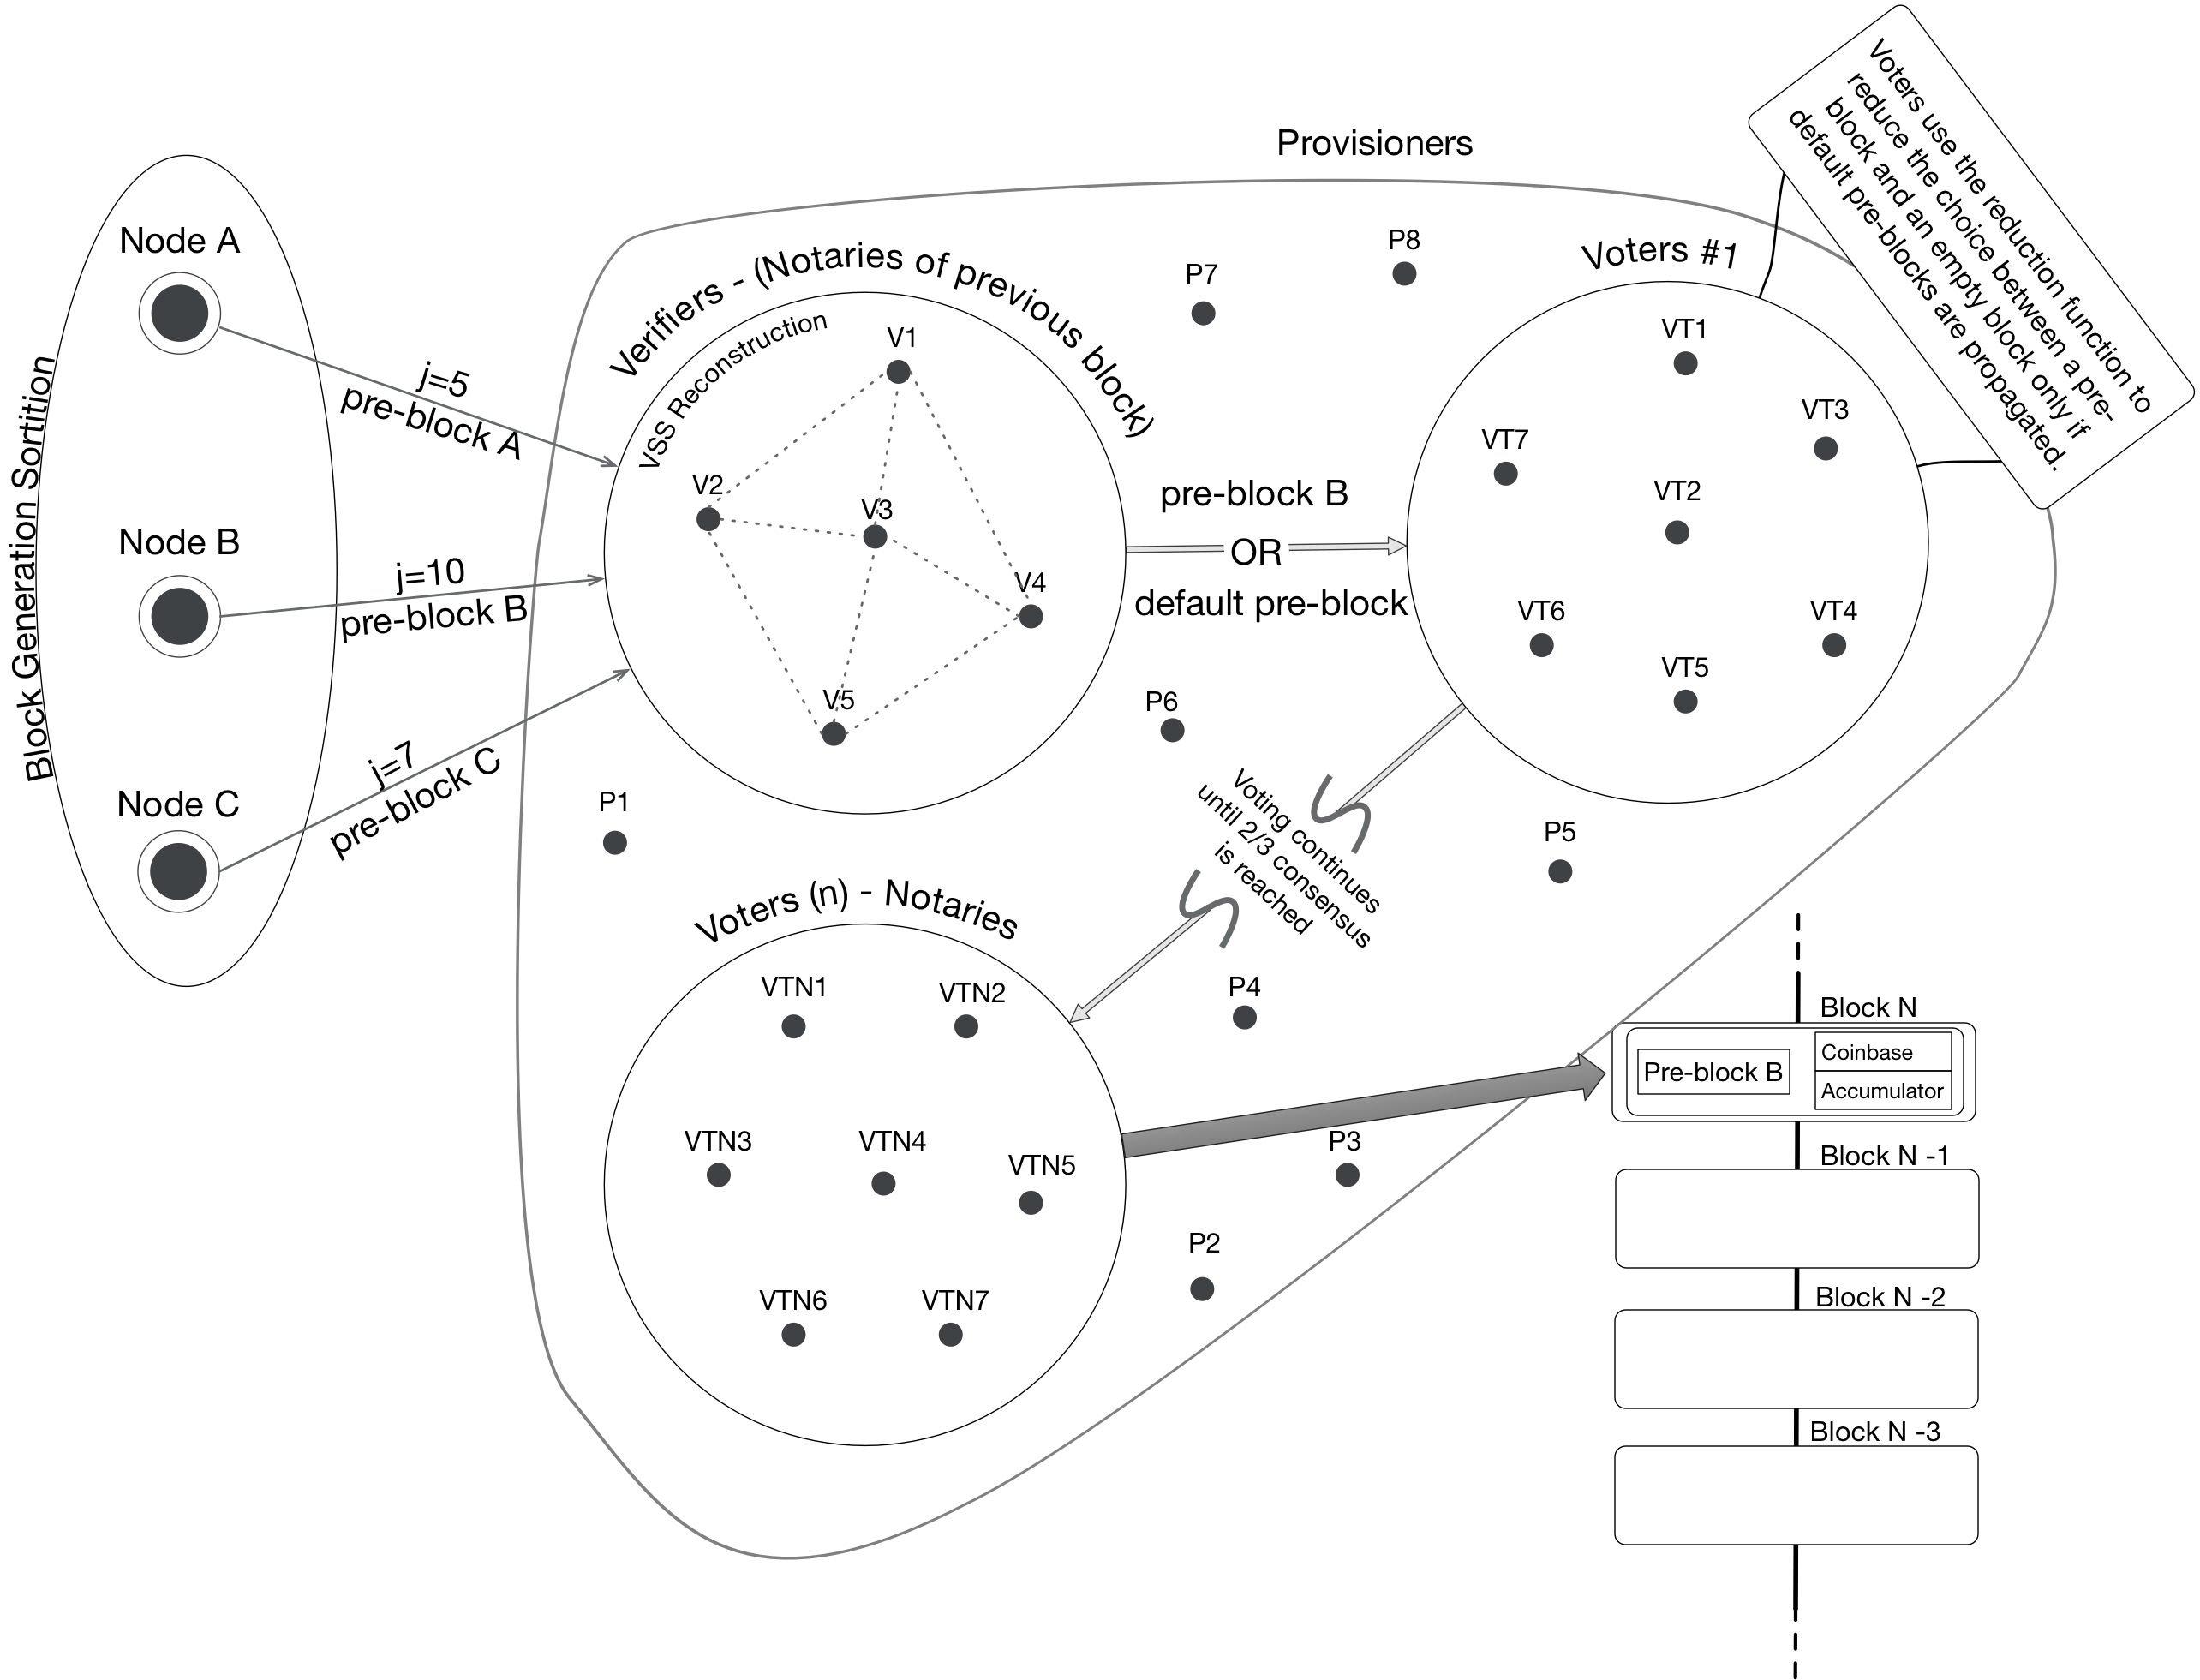
\includegraphics[scale=0.2]{sba}
\caption{SBA$\large\star$ at a glance}
\end{figure*}

\subsection{Voting On Blocks --- Voter's Sortition}

While nodes compete for generating the block, Provisioners other than
the \emph{Verifiers} run the Sortition procedure so to be appointed the
task of \emph{Voters} and reach Byzantine consensus over different
rounds of voting.

Block election happens through a set of steps, each
one requiring a different committee being formed by peers sorted through
VRF output with the voter's role. During each step, sorted nodes (and
only them) gossip their signed hash of the block together with block
round, step in the process and proof of sortition as outputted by the
VRF. Since voting is a task reserved to Provisioners, gossip during this
phase stays confined within the Provisioners' boundaries and is relayed
solely by Voters. As a result, the voting operation completes much
faster than all the others since there is no need to wait 
for messages to reach all extremities of the network.

Provisioners organised in subsequent elected \emph{Voting Committees} try to reach consensus (i.e. counting enough votes for either the pre-block hash or the empty block) by progressively raising the amount of votes for a pre-block or an empty block.

At each subsequent step, the votes cast during the step before remain
accounted for, while the new elected Provisioners cast new votes until
the required majority is reached. Intuitively, the convergence is
guaranteed by the fact that Voters which have already declared consensus
for a pre-block will not vote for any other value in the same round and
will keep proposing the same result until consensus converges.

\subsection{Notaries --- Block Rewards}
\label{sec:Block-Reward}

As soon as the \emph{Validators} reach consensus over a non-empty
\emph{pre-block}, they turn into \emph{Notaries} by running a
supplementary procedure aimed at generating a new block by hashing the
pre-block with a set of \textbf{coin-base} transactions. A
\emph{coin-base transaction} is basically a transaction with no input
which mints new \textrm{Dusk} coins and spend them to the address of the
\emph{Block Generator}.

As opposed to Block Generators, Provisioners do not gain their reward by
winning the sortition procedure. Rather, at the end of each block an
amount of \textrm{Dusk} coins is \emph{coin-based}, dependent on the stake
amount committed by the Provisioner to the Accumulator, independently
from whether they participated in the Block Committee or not. This
amount is thus spent toward the Provisioner's address.

Counterintuitively, the rewards paid are inversely proportional to the
staked amount (i.e. bigger stakes get proportionally less rewarded, in
respect to smaller stakes). This measure is novel and to the writers'
knowledge not a viable option outside of the \textrm{Dusk} Blockchain, where the
probability to win the sortition lottery and therefore take an active
part to the \emph{SBA}\(\large\star\) algorithm is not associated with a
reward, except the sole payment of the transaction fees.

The motivation
is twofold. Together with preventing the \emph{rich get richer} scheme,
the intention is to create a counterposition between \textbf{power}
(intended as the capability to influence block generation by being
selected as part of the Block Committee) and \textbf{money} (intended as
the financial benefit acquired from running Provisioners). Considering
that \emph{SBA}\(\large\star\) is already protected from Sybil attack by
making it probabilistically disadvantageous to dilute a stack into
several balances, similarly, by reversing the proportion between rewards
and stake, the system prevents financially motivated participants to
benefit from organizing themselves into few Provisioner pools at the
expense of decentralization.

\begin{figure}
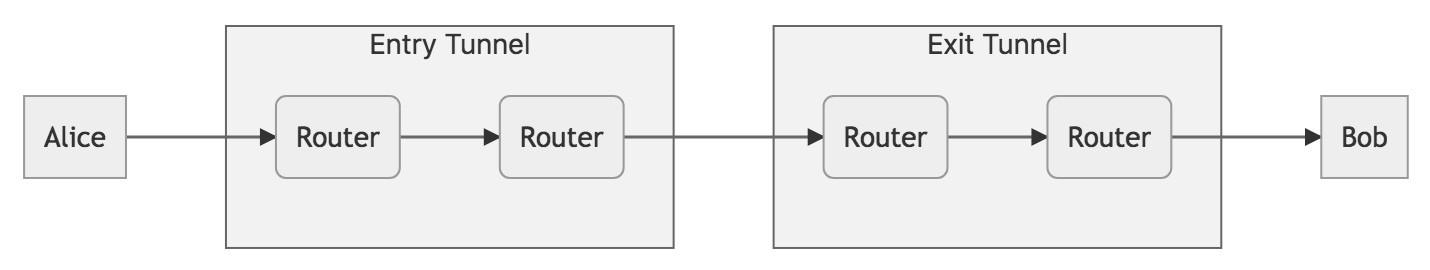
\includegraphics[scale=0.18]{tunnels}
\caption{\textrm{Dusk} tunneling}
\label{tunn}
\end{figure}